\documentclass[19pt]{extarticle}
\usepackage{amsmath,amssymb,amsthm,mathrsfs,amsfonts,dsfont, stmaryrd}
\usepackage[]{algorithm2e}
\usepackage{enumerate}
\usepackage{bm}
\usepackage{graphicx}
\SetKwInOut{Parameter}{Parameters}
\begin{document}

\begin{center}
\huge{PSet Assignment \#1}
\end{center}


\section{Softmax}
\begin{enumerate}[a)]
\item Trivial
\item Code
\end{enumerate}


\section{Neural Network Basics}
\begin{enumerate}[a)]
\item $\forall x \in \mathds{R}\text{, }\sigma(x) = \frac{1}{1 + e^{-x}} $\\
 $\forall x \in \mathds{R}:$
\begin{equation*}\begin{split}
\nabla\sigma(x) &= \frac{e^{-x}}{(1 + e^{-x})^2}\\
&= (\frac{1}{\sigma(x)}-1)\sigma(x)^2\\
&= (1-\sigma(x))\sigma(x)\\
&= \sigma(-x)\sigma(x)\\
\end{split}\end{equation*}


\item $\bm{y} \in \mathds{R}^n$, $\exists k \in \llbracket1,n \rrbracket \quad \bm{y} = \bm{e}_{k}$. Therefore 
$$\forall \bm{\theta} \in  \mathds{R}^n \quad CE(\bm{y},\hat{\bm{y}})= -\log(\hat{y}_k) = - \theta_k + \log(\sum_{i =1}^ne^{\theta_i})$$
Then $\forall \theta \in \mathds{R}^n :$ $$\nabla_{\bm{\theta}} CE (\bm{y},\hat{\bm{y}}) = \hat{\bm{y}} - \bm{y}$$



\item $$\bm{h} = \sigma(\bm{xW}_1 + \bm{b}_1) $$
$$\hat{\bm{y}} = \text{softmax}(\bm{hW}_2 + \bm{b}_2) $$
$\forall \bm{x} \in \mathds{R}^n :$
\begin{equation*}\begin{split}
 \nabla_{\bm{x}} CE(\bm{y},\hat{\bm{y}}) &=\nabla_{\bm{\theta}} CE(\bm{y},\hat{\bm{y}})   (\frac{\partial \bm{\theta}}{\partial \bm{x}})\\
 &\text{ where }\frac{\partial \bm{\theta}}{\partial \bm{x}}\text{ is the Jacobian Matrix : }\\
\forall i \in  \llbracket1,D_y \rrbracket, \forall j \in \llbracket1,D_x \rrbracket \quad (\frac{\partial \bm{\theta}}{\partial \bm{x}})_{ij} &= (\frac{\partial \theta_i}{\partial x_j})\\
 &= (\frac{\partial (\sum_{l = 1}^h h_l(W_2)_{li} + (b_2)_i)}{\partial x_j})\\
  &= (\frac{\partial (\sum_{l = 1}^h \sigma(\sum_{m=1}^{D_x}x_m(W_1)_{ml} +(b_1)_l)(W_2)_{li})}{\partial x_j})\\
    &= (\sum_{l = 1}^h(W_1)_{jl} \sigma'(\sum_{m=1}^{D_x}x_m(W_1)_{ml} +(b_1)_l)(W_2)_{li}))\\
    &= (\bm{W}_1)_{j.}\cdot (\bm{h}'^\top*(\bm{W}_2)_{.i})\\
    &= (\bm{W}_1)_{j.}\cdot (\bm{D}\bm{W}_2)_{.i}\text{ where } \bm{D} = \text{diag}(\sigma '(\bm{xW}_1 + \bm{b}_1))\\
    &= ((\bm{W}_1 \bm{D}\bm{W}_2)^{\top})_{ij}\\
    \\
    \text{ Then } \nabla_{\bm{x}} CE(\bm{y},\hat{\bm{y}}) &= (\hat{\bm{y}} - \bm{y})  \bm{W}_2^{\top} \bm{D}  \bm{W}_1^{\top} \text{ where } \bm{D} = \text{diag}(\sigma '(\bm{xW}_1 + \bm{b}_1))\\
   \end{split}\end{equation*}


\item There are $H(1 + D_x ) + D_y(1 + H)$ parameters. 

\item Code

\item Code

\item 
\begin{equation*}\begin{split}
\nabla_{\bm{W}_2}CE(\bm{y},\hat{\bm{y}}) &= \nabla_{\bm{\theta}} CE(\bm{y},\hat{\bm{y}})   (\frac{\partial \bm{\theta}}{\partial \bm{W}_2})\\
&=\bm{h}^\top (\hat{\bm{y}} - \bm{y}) \\
   \end{split}\end{equation*}
\begin{equation*}\begin{split}
\nabla_{\bm{b}_2}CE(\bm{y},\hat{\bm{y}}) &= \nabla_{\bm{\theta}} CE(\bm{y},\hat{\bm{y}})   (\frac{\partial \bm{\theta}}{\partial \bm{b}_2})\\
&= (\hat{\bm{y}} - \bm{y}) \\
   \end{split}\end{equation*}

\begin{equation*}\begin{split}
\nabla_{\bm{W}_1}CE(\bm{y},\hat{\bm{y}}) &= \nabla_{\bm{\theta}} CE(\bm{y},\hat{\bm{y}})   (\frac{\partial \bm{\theta}}{\partial \bm{W}_1})\\
&=\nabla_{\bm{\theta}} CE(\bm{y},\hat{\bm{y}})   (\frac{\partial \bm{\theta}}{\partial \bm{h}}) (\frac{\partial \bm{h}}{\partial \bm{\bm{W}_1}})\\   
&= \nabla_{\bm{\theta}} CE(\bm{y},\hat{\bm{y}})   \bm{W}_2^\top  (\frac{\partial \bm{h}}{\partial \bm{\bm{W}_1}})\\   
&= \bm{x}^\top \nabla_{\bm{\theta}} CE(\bm{y},\hat{\bm{y}})   \bm{W}_2^\top  \bm{D}
\end{split}\end{equation*}

\begin{equation*}\begin{split}
\nabla_{\bm{b}_1}CE(\bm{y},\hat{\bm{y}}) &= \nabla_{\bm{\theta}} CE(\bm{y},\hat{\bm{y}})   \bm{W}_2^\top  \bm{D}
\end{split}\end{equation*}

\end{enumerate}

\section{ word2vec }
\begin{enumerate}[a)]

\item $\hat{\bm{y}}_o = p(\bm{o}|\bm{c}) = \frac{\exp(\bm{u}_o\bm{v}_c^{\top})}{\sum_{w = 1}^W\exp(\bm{u}_w^{\top}\bm{v}_c)}$.\\
We can rewrite $\hat{y}_o$ as follows : $$\hat{y}_o = \text{softmax}(\bm{v}_c\bm{U}^{\top})_o \quad \text{where }\bm{U}=\begin{pmatrix}
\bm{u}_1\\
.\\
.\\
.\\
.\\
\bm{u}_W\\
\end{pmatrix}$$

Therefore, if $\bm{y} = \bm{e}_o$, then $\forall \bm{ v}_c \in \mathds{R}^n$

\begin{equation*}\begin{split}
\nabla_{\bm{v}_c}CE(\bm{y}, \hat{\bm{y}})&= \nabla_{\bm{v}_c\bm{U}^{\top}}CE(\bm{y}, \hat{\bm{y}})\bm{U}\\
&= (\hat{\bm{y}} - \bm{y})\bm{U}\\
\end{split}\end{equation*}

\item \begin{itemize}
 $\forall w \in \llbracket1, W \rrbracket$ : 
\begin{equation*}\begin{split}
\nabla_{\bm{u}_w}CE(\bm{y}, \hat{\bm{y}})&=(\hat{\bm{y}} - \bm{y})(\frac{\partial (\bm{v}_c\bm{U}^{\top})}{\partial \bm{u}_w})\\
&=  (\hat{\bm{y}} - \bm{y})(\sum_{i = 1}^W\frac{\partial ((\bm{u}_i\bm{v}_c^{\top})\bm{e}_i)}{\partial \bm{u}_w})^{\top}\\
&=(\hat{y}_w - y_w)\cdot \bm{v}_c\\
&=  (\hat{y}_w - \delta_{wo})\cdot \bm{v}_c\\
\end{split}\end{equation*}

\end{itemize}


\item Now $J_{\text{neg-sample}}(\bm{o}, \bm{v}_c, \bm{U}) = - \log((\sigma(\bm{u}_o\bm{v}_c^{\top}))
- \sum_{k=1}^K\log(\sigma(-\bm{u}_k\bm{v}_c^{\top}))$
\begin{itemize}
\item  $\forall \bm{ v}_c \in \mathds{R}^n$

\begin{equation*}\begin{split}
\nabla_{\bm{v}_c}CE(\bm{y}, \hat{\bm{y}}) &=-\frac{\sigma(-\bm{u}_o\bm{v}_c^{\top})\sigma(\bm{u}_o\bm{v}_c^{\top})}{\sigma(\bm{u}_o\bm{v}_c^{\top})}\bm{u}_o + \sum_{k=1}^K\frac{\sigma(-\bm{u}_k\bm{v}_c^{\top})\sigma(\bm{u}_k\bm{v}_c^{\top})}{\sigma(-\bm{u}_k\bm{v}_c^{\top})}\bm{u}_k\\
&=-\sigma(-\bm{u}_o\bm{v}_c^{\top})\bm{u}_o + \sum_{k=1}^K\sigma(\bm{u}_k\bm{v}_c^{\top})\bm{u}_k\\
\end{split}\end{equation*}

\item If $w \neq o$ : 
\begin{equation*}\begin{split}
\nabla_{\bm{u}_w}CE(\bm{y}, \hat{\bm{y}})&= \sigma(\bm{u}_w\bm{v}_c^{\top})\bm{v}_c\\
\end{split}\end{equation*}

\item If $w = o$ : 
\begin{equation*}\begin{split}
\nabla_{\bm{u}_o}CE(\bm{y}, \hat{\bm{y}})&= -\sigma(-\bm{u}_o\bm{v}_c^{\top})\bm{v}_c\\
&= (\sigma(\bm{u}_o\bm{v}_c^{\top}) -1)\bm{v}_c
\end{split}\end{equation*}

Conclusion : $\forall w \in \llbracket1, W \rrbracket$ : 
$$\nabla_{\bm{u}_w}CE(\bm{y}, \hat{\bm{y}}) =  (\sigma(\bm{u}_w\bm{v}_c^{\top}) -\delta_{wo})\bm{v}_c$$


\end{itemize}


\item $J_{\text{skip-gram}}(\text{word}_{c-m...c+m}) = \sum_{-m\leq j\leq m,j\neq 0}F(\bm{w}_{c+j} , \bm{v}_c)$

\begin{itemize}
\item  $\forall \bm{ v}_c \in \mathds{R}^n$
\begin{equation*}\begin{split}
\nabla_{\bm{v}_c}J &= \sum_{-m\leq j\leq m,j\neq 0}\frac{\partial F(\bm{w}_{c+j} , \bm{v}_c)}{\partial \bm{v}_c} \\
\end{split}\end{equation*}
\item \begin{equation*}\begin{split}
\nabla_{\bm{u}_w}J&= \sum_{-m\leq j\leq m,j\neq 0}\frac{\partial F(\bm{w}_{c+j} , \bm{v}_c)}{\partial \bm{u}_w} \\
\end{split}\end{equation*}

\end{itemize}

$$J_\text{CBOW}(\text{word}_{c-m...c+m}) = F(\bm{w}_c, \hat{\bm{v}}) \text{ with }\hat{\bm{v}} = \sum_{
-m\leq j \leq m,j\neq 0}
\bm{v}_{c+j}$$
\begin{itemize}
\item 
\begin{equation*}\begin{split}
\nabla_{\bm{v}_c}J &= \vec{0} \\
\end{split}\end{equation*}

\item \begin{equation*}\begin{split}
\nabla_{\bm{u}_w}J&=\frac{\partial  F(\bm{w}_c, \hat{\bm{v}})}{\partial \bm{w}_c}\frac{\partial \bm{w}_c}{\partial \bm{u}_w} \\
\end{split}\end{equation*}

\end{itemize}

\item Code

\item Code

\item Code

\item 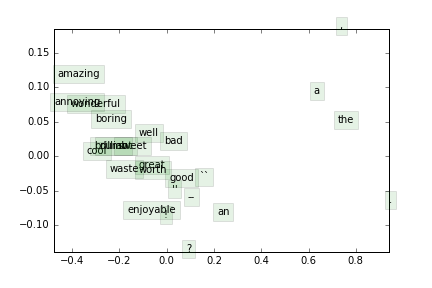
\includegraphics{q3_word_vectors.png}

\end{enumerate}


\section{ Sentiment Analysis}


\begin{enumerate}[a)]
\item $J = \frac{1}{N}\sum_{i=1}^NCE(\hat{\bm{y}}_i,\bm{y}_i) + \frac{\lambda}{2}\|\bm{W}\|^2$ with $\hat{\bm{y}_i} = \text{softmax}(\bm{x}_i\bm{W})$\\
$\forall\text{ } \bm{W}$: 
 \begin{equation*}\begin{split}
\nabla_{\bm{W}}J &= \frac{1}{N}\sum_{i=1}^N\nabla_{\bm{W}}CE(\hat{\bm{y}}_i,\bm{y}_i) + \frac{\lambda}{2}\nabla_{\bm{W}}\|\bm{W}\|^2\\
&= \frac{1}{N}\sum_{i=1}^N\bm{x}_i^\top(\hat{\bm{y}}_i-\bm{y}_i) + \lambda\bm{W}\\
\end{split}\end{equation*}


\item Blah blah blah ... OverFitting ... Blah blah blah more Bias for less Variance  ... Blah blah blah

\item I selected $\lambda \in \{ 0.1, 0.01, 0.01, 0.001, 0.0001\}$

\item 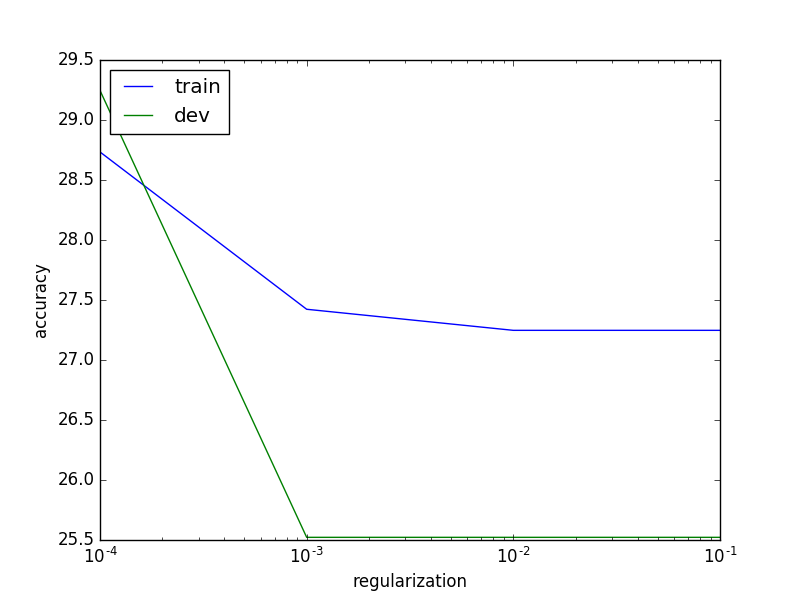
\includegraphics{q4_reg_v_acc.png}
\end{enumerate}




\end{document}